\documentclass{beamer}
\usepackage{amsmath}
\usepackage[english]{babel} %set language; note: after changing this, you need to delete all auxiliary files to recompile
\usepackage[utf8]{inputenc} %define file encoding; latin1 is the other often used option
\usepackage{csquotes} % provides context sensitive quotation facilities
\usepackage{graphicx} %allows for inserting figures
\usepackage{booktabs} % for table formatting without vertical lines
\usepackage{textcomp} % allow for example using the Euro sign with \texteuro
\usepackage{stackengine}
\usepackage{wasysym}
\usepackage{tikzsymbols}
\usepackage{textcomp}
\newcommand{\bubblethis}[2]{
        \tikz[remember picture,baseline]{\node[anchor=base,inner sep=0,outer sep=0]%
        (#1) {\underline{#1}};\node[overlay,cloud callout,callout relative pointer={(0.2cm,-0.7cm)},%
        aspect=2.5,fill=yellow!90] at ($(#1.north)+(-0.5cm,1.6cm)$) {#2};}%
    }%
\tikzset{face/.style={shape=circle,minimum size=4ex,shading=radial,outer sep=0pt,
        inner color=white!50!yellow,outer color= yellow!70!orange}}
%% Some commands to make the code easier
\newcommand{\emoticon}[1][]{%
  \node[face,#1] (emoticon) {};
  %% The eyes are fixed.
  \draw[fill=white] (-1ex,0ex) ..controls (-0.5ex,0.2ex)and(0.5ex,0.2ex)..
        (1ex,0.0ex) ..controls ( 1.5ex,1.5ex)and( 0.2ex,1.7ex)..
        (0ex,0.4ex) ..controls (-0.2ex,1.7ex)and(-1.5ex,1.5ex)..
        (-1ex,0ex)--cycle;}
\newcommand{\pupils}{
  %% standard pupils
  \fill[shift={(0.5ex,0.5ex)},rotate=80] 
       (0,0) ellipse (0.3ex and 0.15ex);
  \fill[shift={(-0.5ex,0.5ex)},rotate=100] 
       (0,0) ellipse (0.3ex and 0.15ex);}

\newcommand{\emoticonname}[1]{
  \node[below=1ex of emoticon,font=\footnotesize,
        minimum width=4cm]{#1};}
\usepackage{scalerel}
\usetikzlibrary{positioning}
\usepackage{xcolor,amssymb}
\newcommand\dangersignb[1][2ex]{%
  \scaleto{\stackengine{0.3pt}{\scalebox{1.1}[.9]{%
  \color{red}$\blacktriangle$}}{\tiny\bfseries !}{O}{c}{F}{F}{L}}{#1}%
}
\newcommand\dangersignw[1][2ex]{%
  \scaleto{\stackengine{0.3pt}{\scalebox{1.1}[.9]{%
  \color{red}$\blacktriangle$}}{\color{white}\tiny\bfseries !}{O}{c}{F}{F}{L}}{#1}%
}
\usepackage{fontawesome} % Social Icons
\usepackage{epstopdf} % allow embedding eps-figures
\usepackage{tikz} % allows drawing figures
\usepackage{amsmath,amssymb,amsthm} %advanced math facilities
\usepackage{lmodern} %uses font that support italic and bold at the same time
\usepackage{hyperref}
\usepackage{tikz}
\hypersetup{
    colorlinks=true,
    linkcolor=blue,
    filecolor=magenta,      
    urlcolor=blue,
}
\usepackage{tcolorbox}
%add citation management using BibLaTeX
\usepackage[citestyle=authoryear-comp, %define style for citations
    bibstyle=authoryear-comp, %define style for bibliography
    maxbibnames=10, %maximum number of authors displayed in bibliography
    minbibnames=1, %minimum number of authors displayed in bibliography
    maxcitenames=3, %maximum number of authors displayed in citations before using et al.
    minnames=1, %maximum number of authors displayed in citations before using et al.
    datezeros=false, % do not print dates with leading zeros
    date=long, %use long formats for dates
    isbn=false,% show no ISBNs in bibliography (applies only if not a mandatory field)
    url=false,% show no urls in bibliography (applies only if not a mandatory field)
    doi=false, % show no dois in bibliography (applies only if not a mandatory field)
    eprint=false, %show no eprint-field in bibliography (applies only if not a mandatory field)
    backend=biber %use biber as the backend; backend=bibtex is less powerful, but easier to install
    ]{biblatex}
\addbibresource{../mybibfile.bib} %define bib-file located one folder higher


\usefonttheme[onlymath]{serif} %set math font to serif ones

\definecolor{beamerblue}{rgb}{0.2,0.2,0.7} %define beamerblue color for later use

%%% defines highlight command to set text blue
\newcommand{\highlight}[1]{{\color{blue}{#1}}}


%%%%%%% commands defining backup slides so that frame numbering is correct

\newcommand{\backupbegin}{
   \newcounter{framenumberappendix}
   \setcounter{framenumberappendix}{\value{framenumber}}
}
\newcommand{\backupend}{
   \addtocounter{framenumberappendix}{-\value{framenumber}}
   \addtocounter{framenumber}{\value{framenumberappendix}}
}

%%%% end of defining backup slides

%Specify figure caption, see also http://tex.stackexchange.com/questions/155738/caption-package-not-working-with-beamer
\setbeamertemplate{caption}{\insertcaption} %redefines caption to remove label "Figure".
%\setbeamerfont{caption}{size=\scriptsize,shape=\itshape,series=\bfseries} %sets figure  caption bold and italic and makes it smaller


\usetheme{Boadilla}

%set options of hyperref package
\hypersetup{
    bookmarksnumbered=true, %put section numbers in bookmarks
    naturalnames=true, %use LATEX-computed names for links
    citebordercolor={1 1 1}, %color of border around cites, here: white, i.e. invisible
    linkbordercolor={1 1 1}, %color of border around links, here: white, i.e. invisible
    colorlinks=true, %color links
    anchorcolor=black, %set color of anchors
    linkcolor=beamerblue, %set link color to beamer blue
    citecolor=blue, %set cite color to beamer blue
    pdfpagemode=UseThumbs, %set default mode of PDF display
    breaklinks=true, %break long links
    pdfstartpage=1 %start at first page
    }


% --------------------
% Overall information
% --------------------
\title[Economía I]{Economía I \vspace{4mm}
\\ Magistral 24: Mercado de dinero II}
\date{}
\author[Ertola Navajas y Fariña]{Ertola Navajas y Fariña}
\vspace{0.4cm}
\institute[]{Universidad de San Andrés} 


\begin{document}

\begin{frame}
\titlepage
\centering
Magistral 24


\includegraphics[scale=0.2]{Slides Principios de Economia/Figures/logoUDESA.jpg} 
\end{frame}



\begin{frame}{La teoría cuantitativa del dinero}
\begin{itemize}
        \item La teoría cuantitativa del dinero
        \vspace{0.3cm}
                \begin{tcolorbox}[width=4in,
                  interior hidden,
                  boxsep=0pt,
                  left=0pt,
                  right=0pt,
                  top=2pt,
                  ]%%
                                 $$M*V(i)=P*Y$$
                \end{tcolorbox} 
        \item Si el producto está dado por el mercado de trabajo y la tasa de interés por el mercado de crédito
        \item La ecuación se transforma en una ecuación de determinación de los precios
    \end{itemize}
    \begin{itemize}
    \begin{tcolorbox}[width=4in,
                  interior hidden,
                  boxsep=0pt,
                  left=0pt,
                  right=0pt,
                  top=2pt,
                  ]%%
                                 $$P=\left(\frac{M^{*} V}{Y}\right)$$
                \end{tcolorbox} 
    \end{itemize}
    \begin{itemize}
        \item Aumentos en \textit{M} son seguidos por aumentos en \textit{P}
    \end{itemize}
\end{frame}

\begin{frame}{Inflación}
    \begin{itemize}
    \item La TCD con tasas de crecimiento: \\
$$\frac{\vartriangle M}{M} + \frac{\vartriangle V}{V} = \frac{\vartriangle P}{P} + \frac{\vartriangle Y}{Y}$$ \vspace{1mm}
    \item Sabiendo que la inflación es $\pi = \frac{\vartriangle P}{P}$, luego la inflación es: \\
    $$\pi = \frac{\vartriangle M}{M} - \frac{\vartriangle Y}{Y} + \frac{\vartriangle V}{V}$$ \vspace{1mm}
    \item La tasa de crecimiento del dinero es un predictor esencial de la inflación
    %\item Y consecuentemente también lo son los déficit fiscales u otro motivo de expansión monetaria
    \end{itemize}
\end{frame}

\begin{frame}{Evolución de la base monetaria vs. IPC}
\centering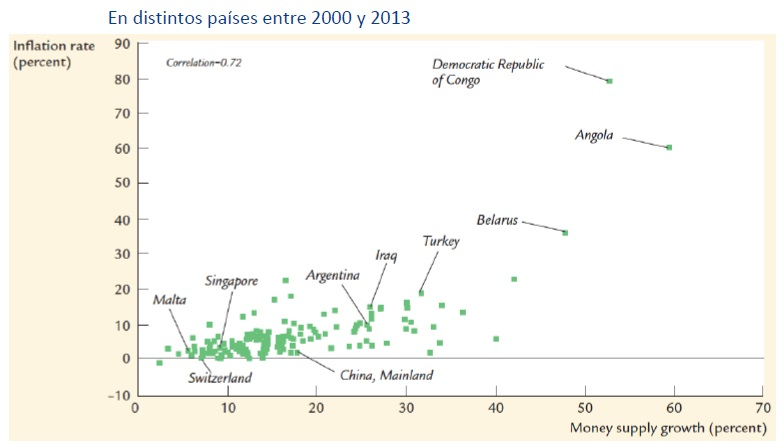
\includegraphics[width=11cm]{Slides Principios de Economia/Figures/C33.4.jpg}\
\end{frame}

\begin{frame}{Evolución de la base monetaria vs. IPC}
\centering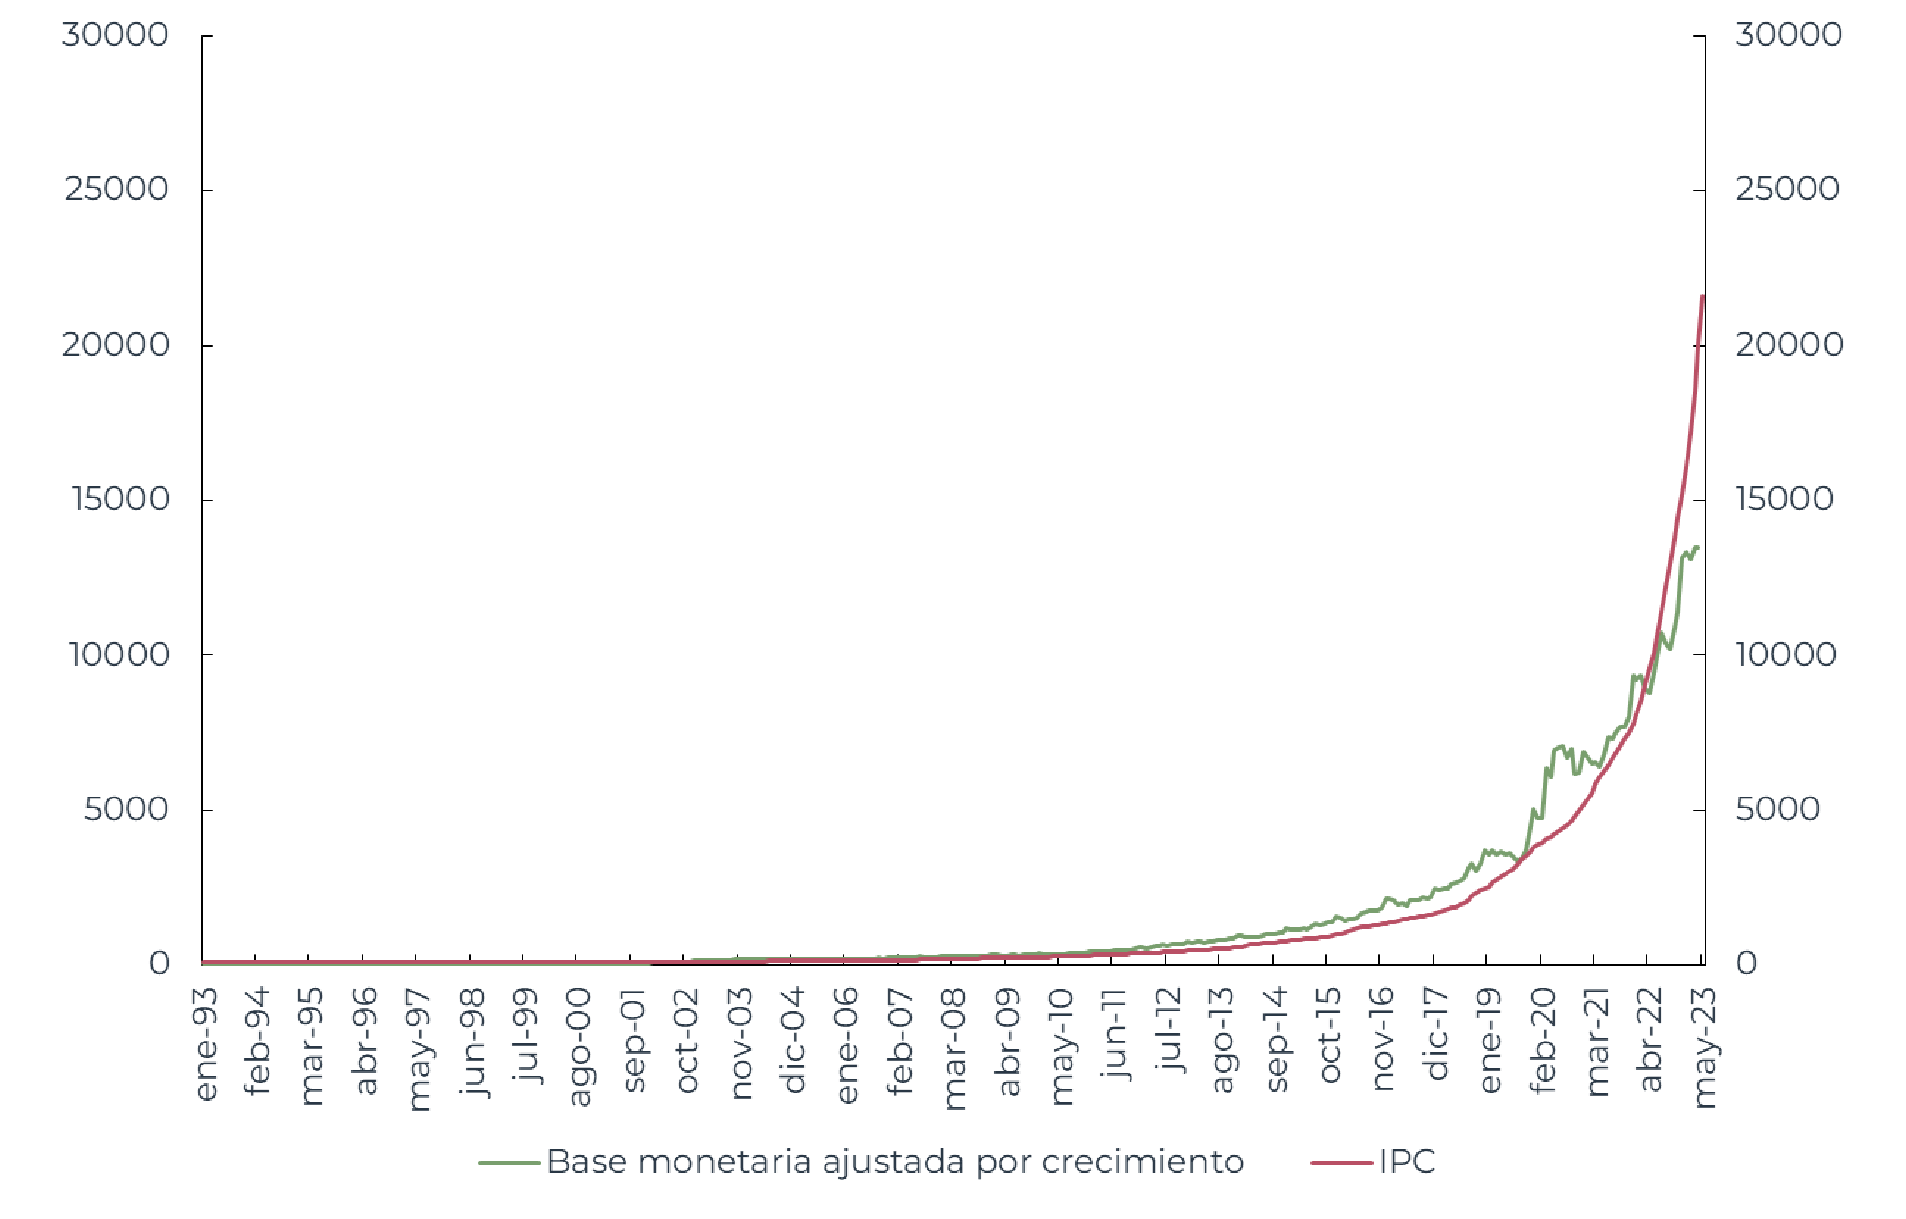
\includegraphics[width=11cm]{Slides Principios de Economia/Figures/38.7 (1).pdf}\
\end{frame}

\begin{frame}{El equilibrio del mercado monetario}
\centering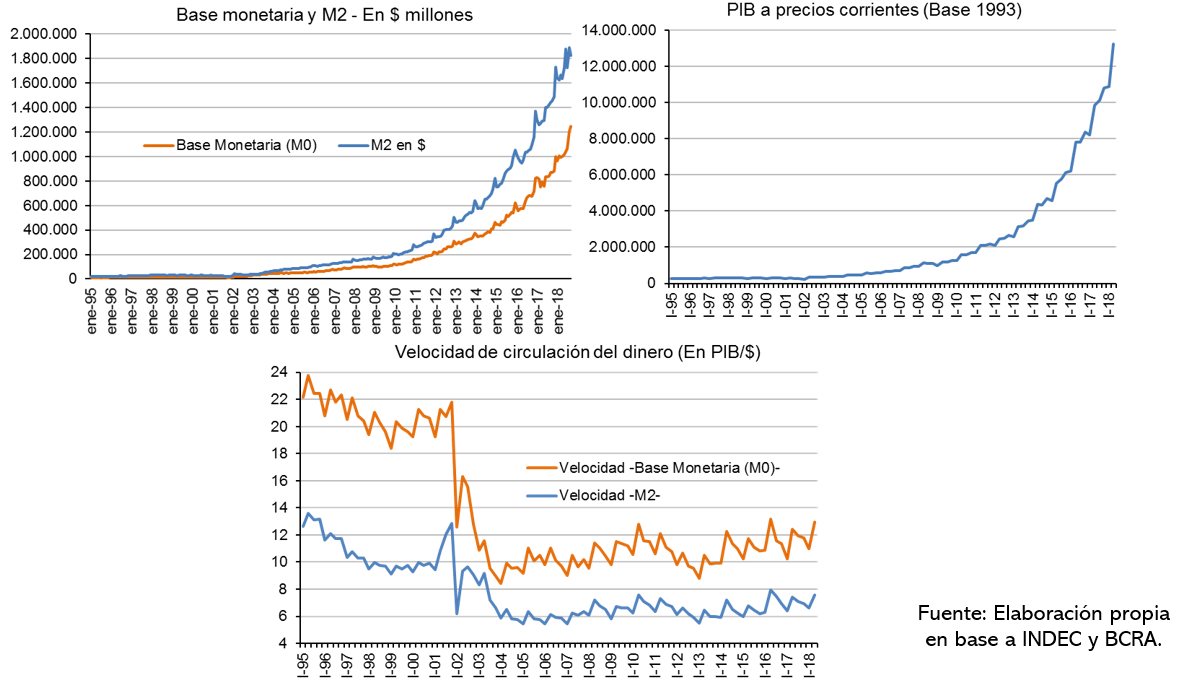
\includegraphics[width=11cm]{Slides Principios de Economia/Figures/P56.png}\
\end{frame}

\begin{frame}{El equilibrio del mercado monetario II}
\centering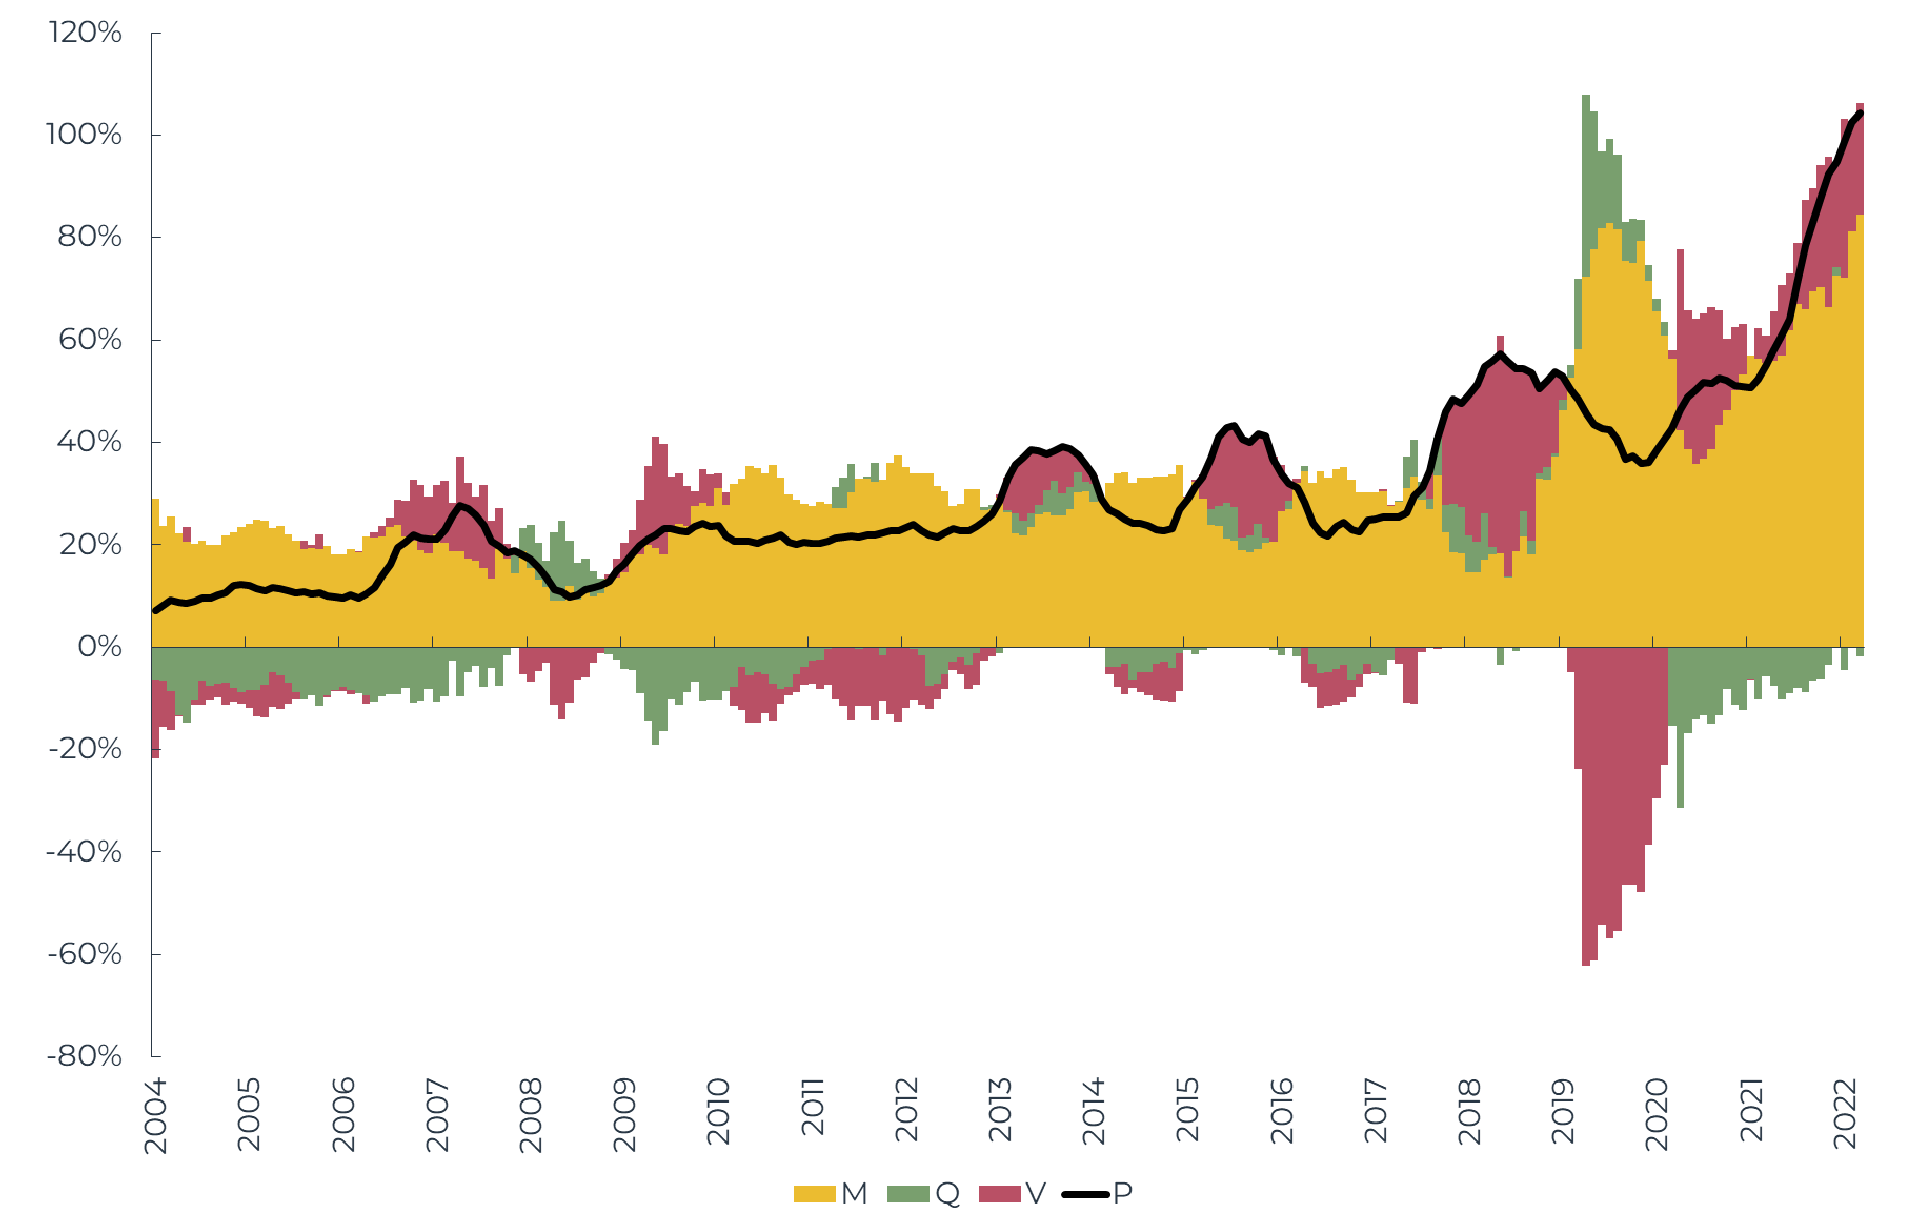
\includegraphics[width=10cm]{Slides Principios de Economia/Figures/38.9.pdf}\
\end{frame}

\begin{frame}{Malas teorías de la inflación}
    \begin{itemize}
        \item Realmente solo en Argentina se repiten estas ideas
            \begin{itemize}
        \item Es la puja distributiva
        \item Es culpa del dolar
        \item El aumento de las tarifas como generadoras de inflación
        \item Los supermercados aumentan los márgenes de ganancia y eso explica por qué aumentan los precios
            \end{itemize}
        \item Ninguna de estas teorías puede explicar la inflación
        \item Obviamente se mueven con la inflación y por eso es fácil confundirse, recuerden el problema de la variable omitida
        \item Y todo esto puede afectar las expectativas que se forman las personas acerca de los precios y, se complica más la cosa
        \item Por ejemplo: si las expectativas no se alinean, la política monetaria va a tener que ser más dura para bajar la inflación
    \end{itemize}
\end{frame}

\begin{frame}{La relación entre política monetaria y precios...}
\centering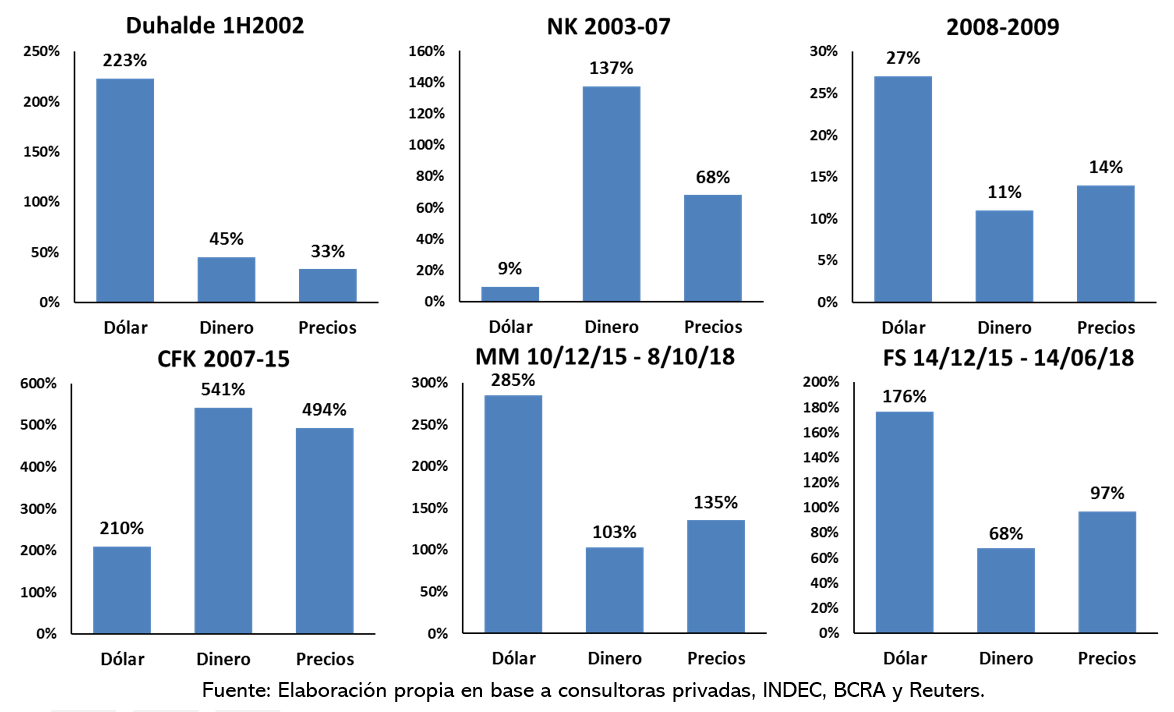
\includegraphics[width=11cm]{Slides Principios de Economia/Figures/P57.png}\
\end{frame}

\begin{frame}{La relación entre tarifas e inflación...}
\centering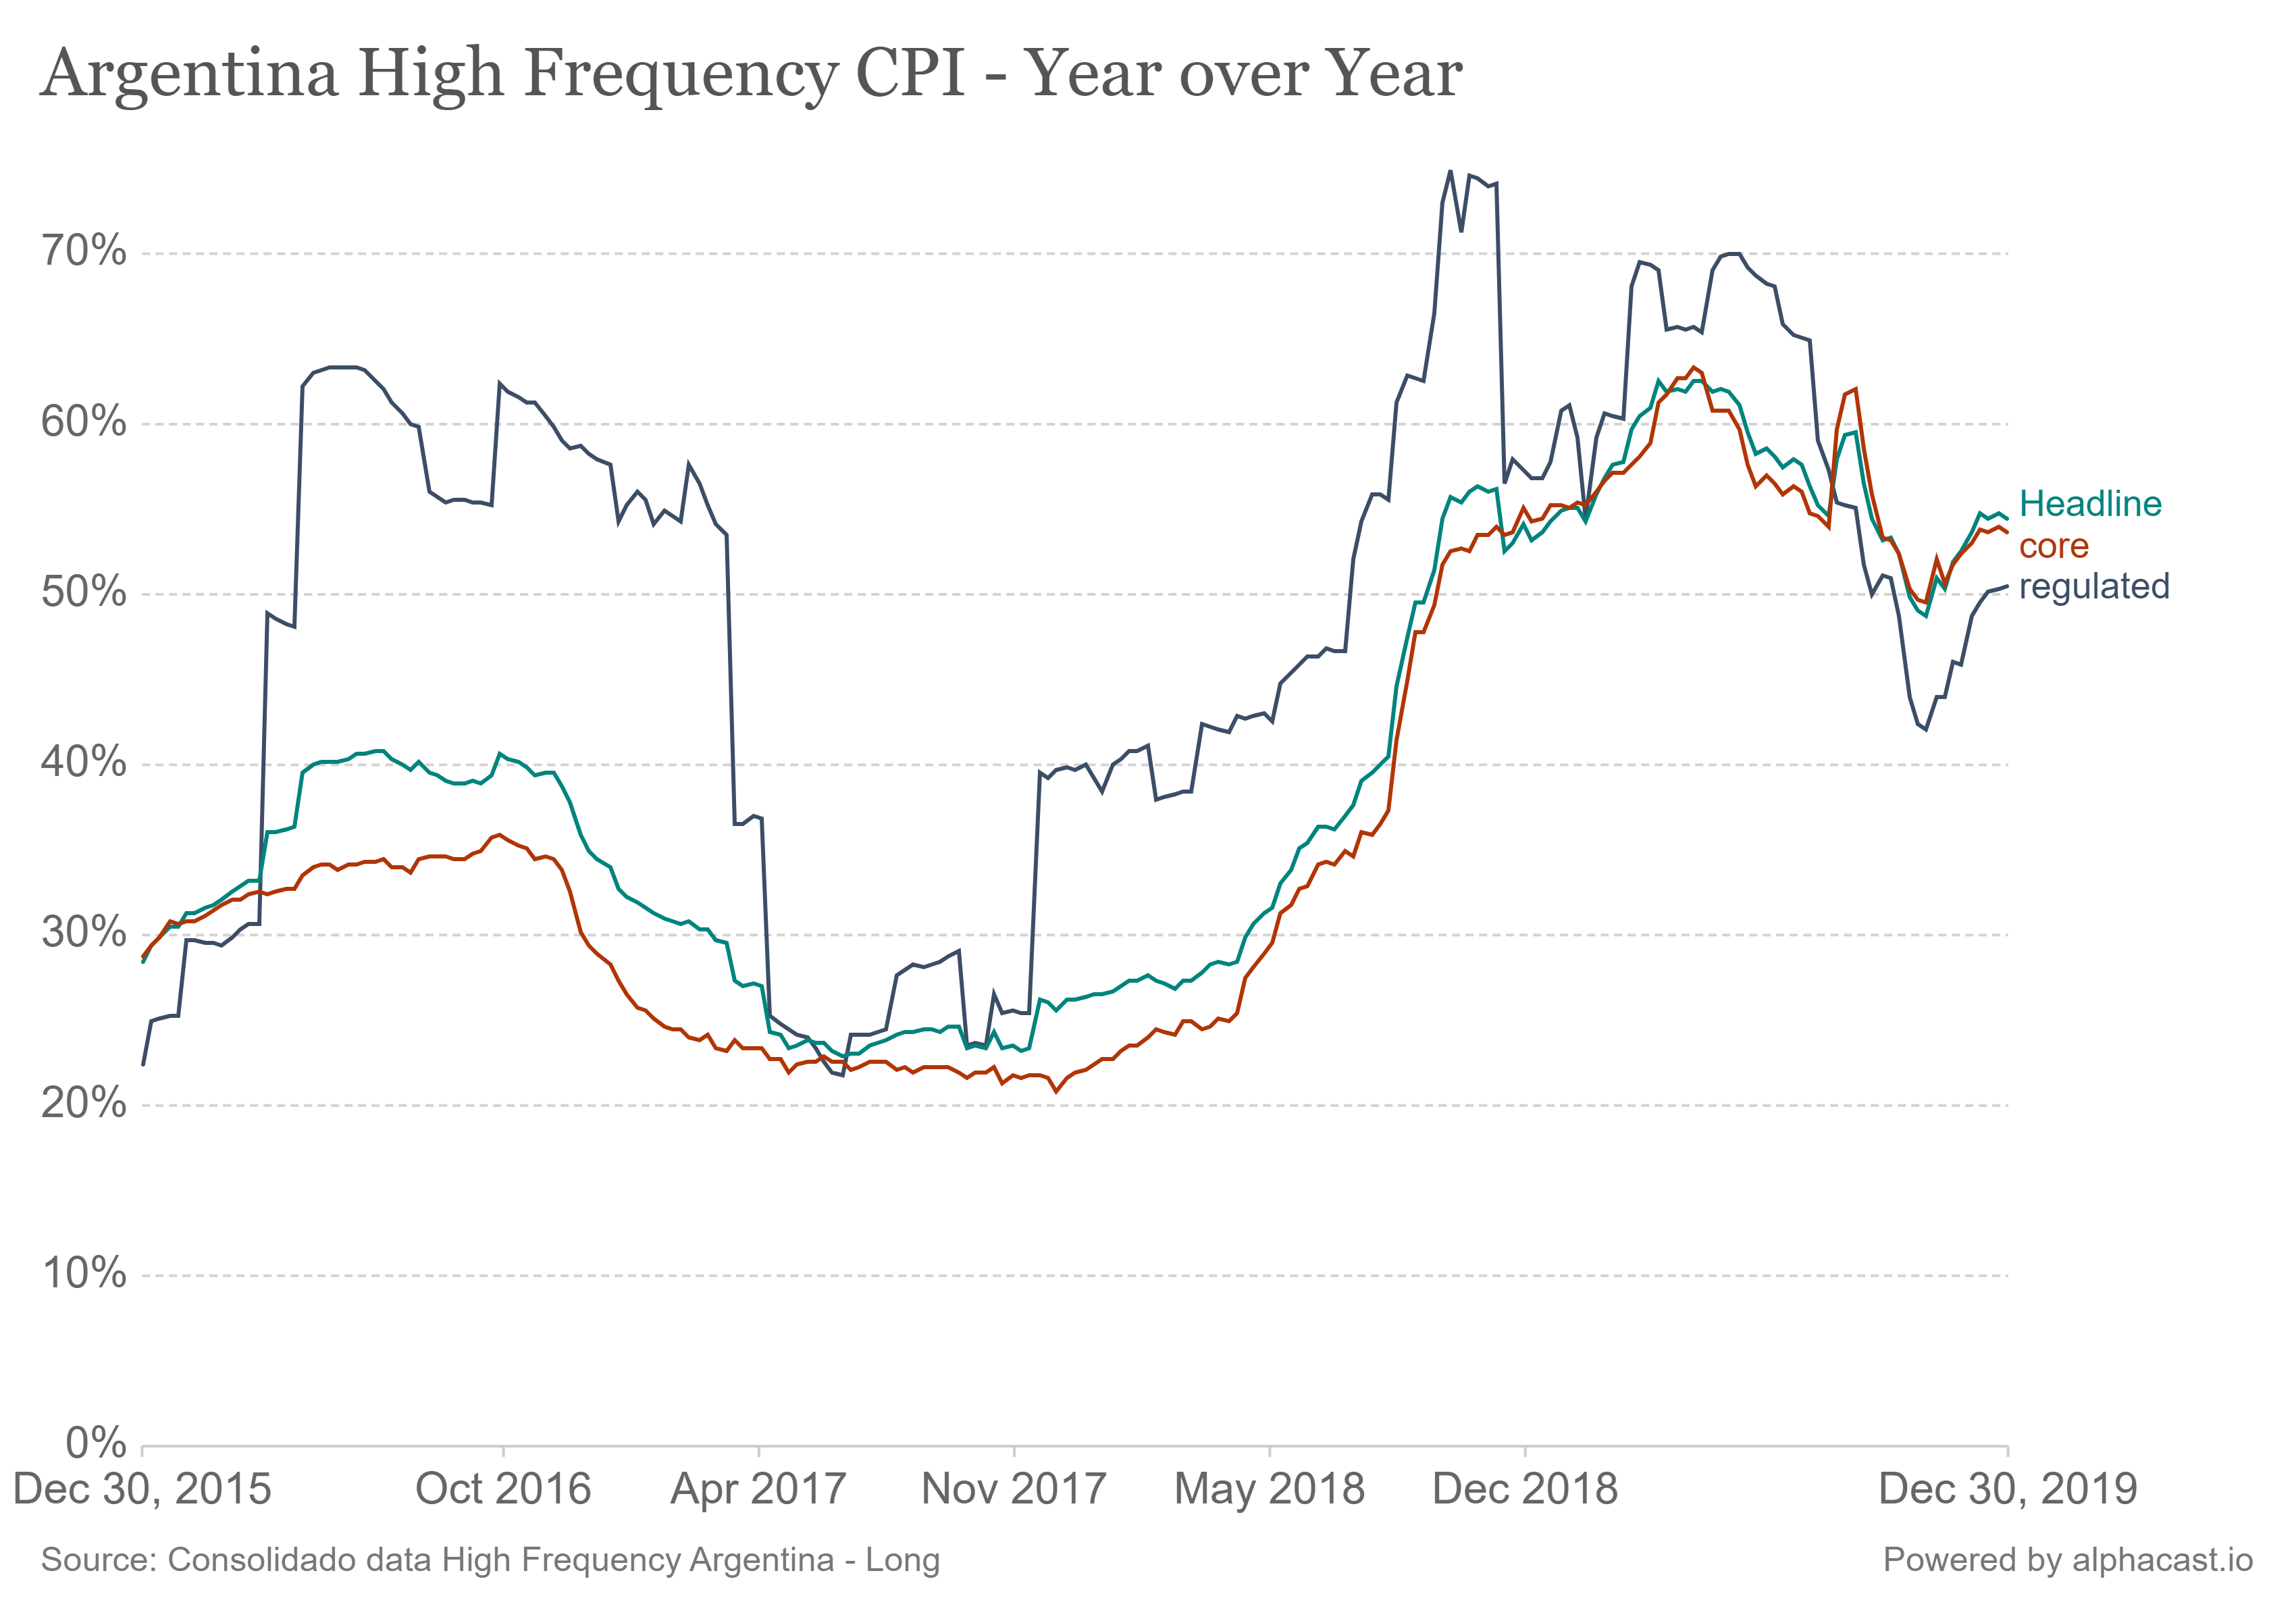
\includegraphics[width=11cm]{Slides Principios de Economia/Figures/G20.png}\
\end{frame}


\begin{frame}
\frametitle{¿Por qué emitir dinero!?}
\begin{itemize}
    \item La inflación puede funcionar como variable de ajuste \vspace{2mm}
    \item El gobierno se queda con el impuesto inflacionario
    \begin{itemize}
        \item Al emitir dinero, el gobierno hace que el salario de la gente valga menos
    \end{itemize}
    \item La particularidad del impuesto inflacionario es que no parte de un debate y posterior aprobación en la Cámara de Diputados. Es un impuesto oculto que se cobra sin decir que es cobrado.
\end{itemize}
\end{frame}

\begin{frame}
\frametitle{¿Cómo funciona el impuesto inflacionario?}
\begin{itemize}
    \item El gobierno le debe pagar a Gaby y a Maxi \$100 a cada uno. 
    \item Por otro lado, en la economía hay 20 flynn paffs. Precio de un flynn paff: \$5.
    \item Solo tiene \$100 y se los da a Gaby. ¿Y a Maxi? ¡A imprimir!
    \item Ahora hay \$200 dando vueltas, pero los mismos 20 flynn paffs. Precio de un flynn paff: \$10
    \item Conclusión: ¡Cada uno puede comprar 10!
\end{itemize}
\end{frame}

\begin{frame}
\frametitle{Emisión y señoreaje}
\begin{itemize}
    \item Recordemos que los gobiernos pueden financiarse imprimiendo dinero
        \begin{itemize}
        \item Bonos que el Banco Central se ve obligado a aceptar \\
        - Monetización de la deuda
        \end{itemize}
    \vspace{2mm}
    \item Uso del señoreaje
\begin{itemize}
        \item Retorno por la creación de dinero
        \item Como la expansión monetaria típicamente conlleva a una subida de precios, funciona como un impuesto inflacionario sobre tenedores de dinero 
        \end{itemize}
\end{itemize}
\end{frame}

\begin{frame}{Efectos negativos}
    \begin{itemize}
 \item Rompe el sistema de precios
 \item Dificultad para establecer contratos de largo plazo, algo central en cualquier economía moderna.
 \item  Obliga a las personas a economizar el uso del dinero,
algo que los economistas llaman el costo de suela de zapatos
\item Menor crecimiento
  \end{itemize}
\end{frame}

\begin{frame}{Efectos negativos}
\centering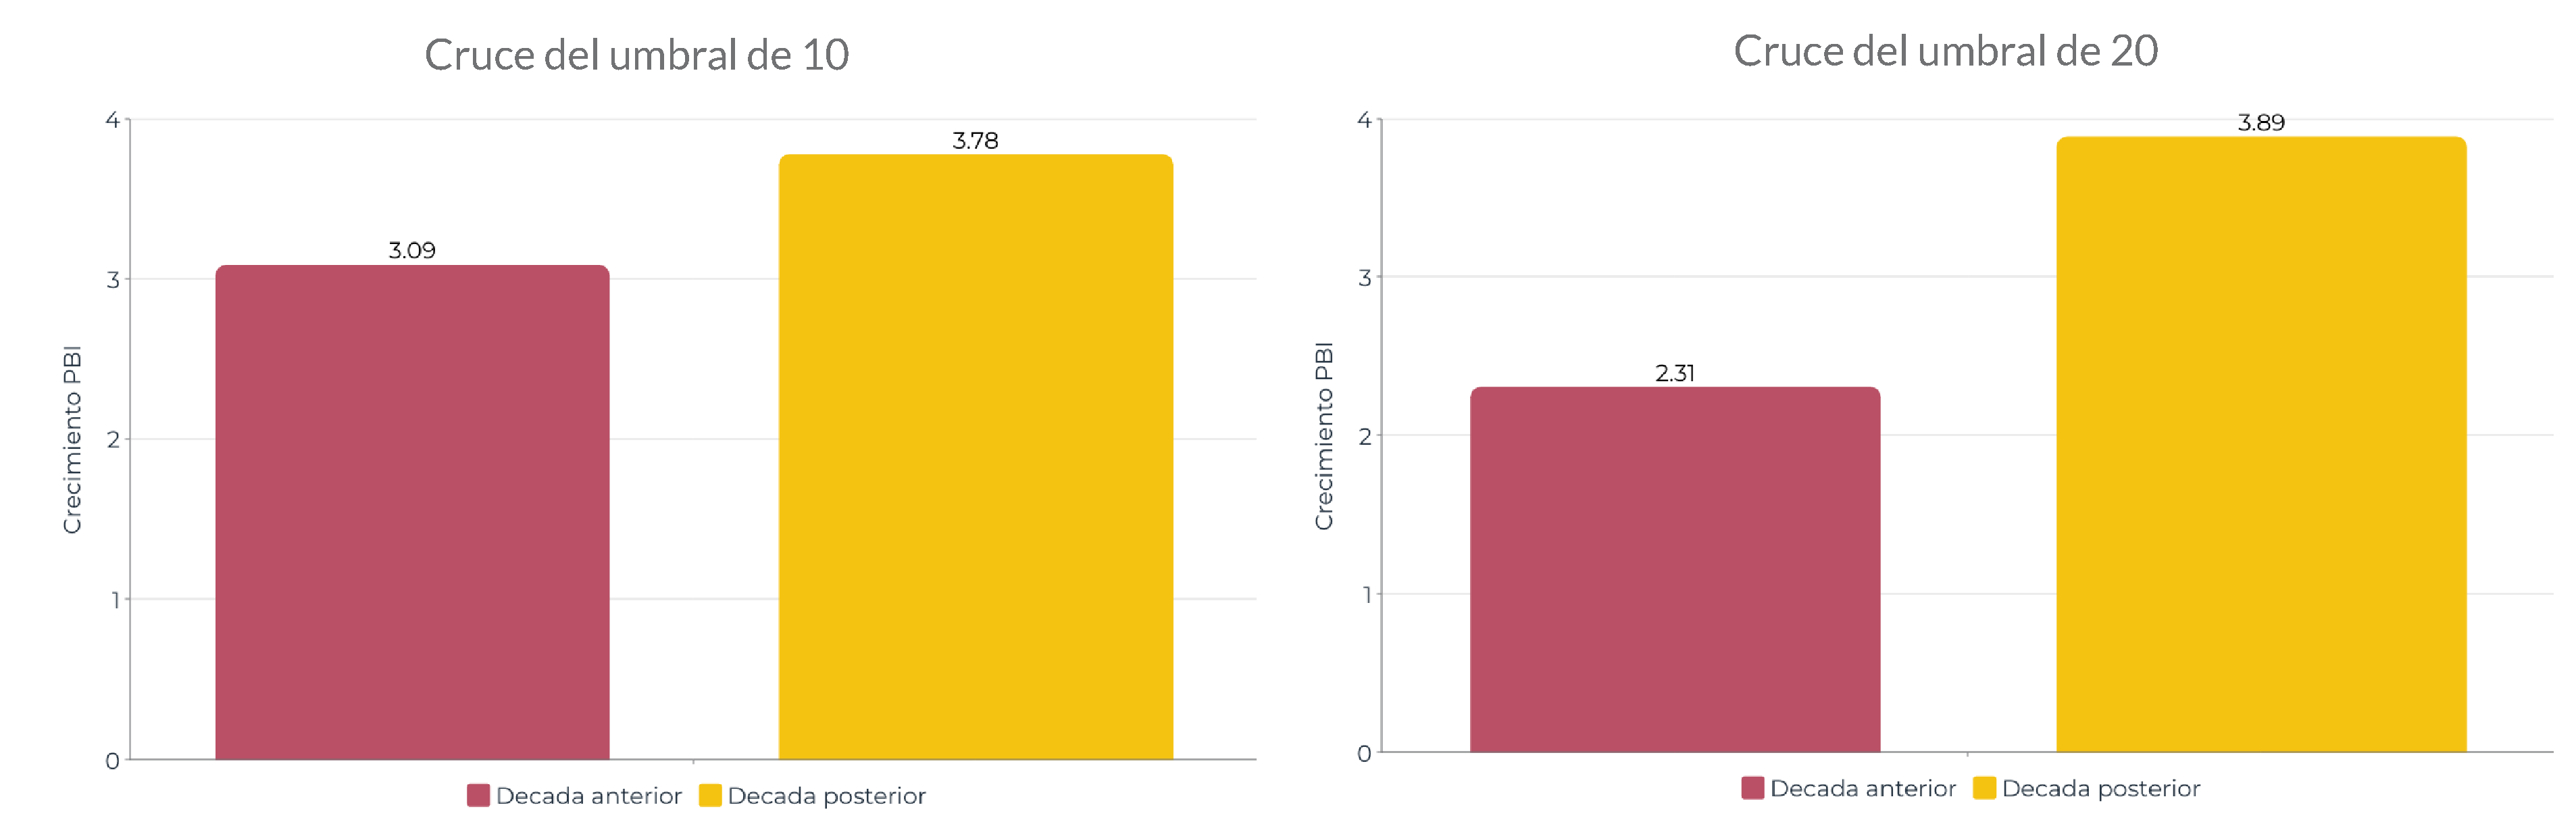
\includegraphics[width=11cm]{Slides Principios de Economia/Figures/38.11.pdf}\
\end{frame}

\begin{frame}{La inflación en el mundo}
    \centering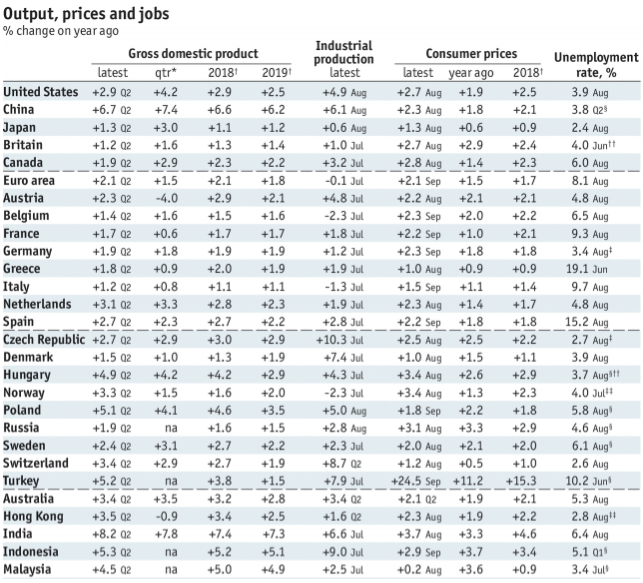
\includegraphics[width=8cm]{Slides Principios de Economia/P70.png}\
\end{frame}


\begin{frame}{Continuación}
    \centering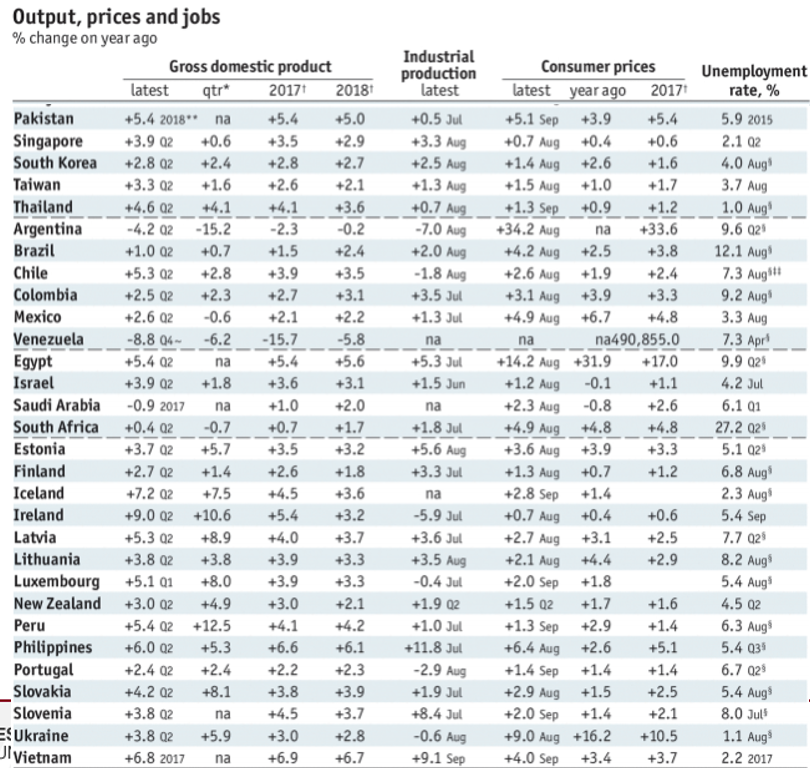
\includegraphics[width=8cm]{Slides Principios de Economia/P71.png}\
\end{frame}

\begin{frame}{La inflación en Argentina en una perspectiva histórica}
\centering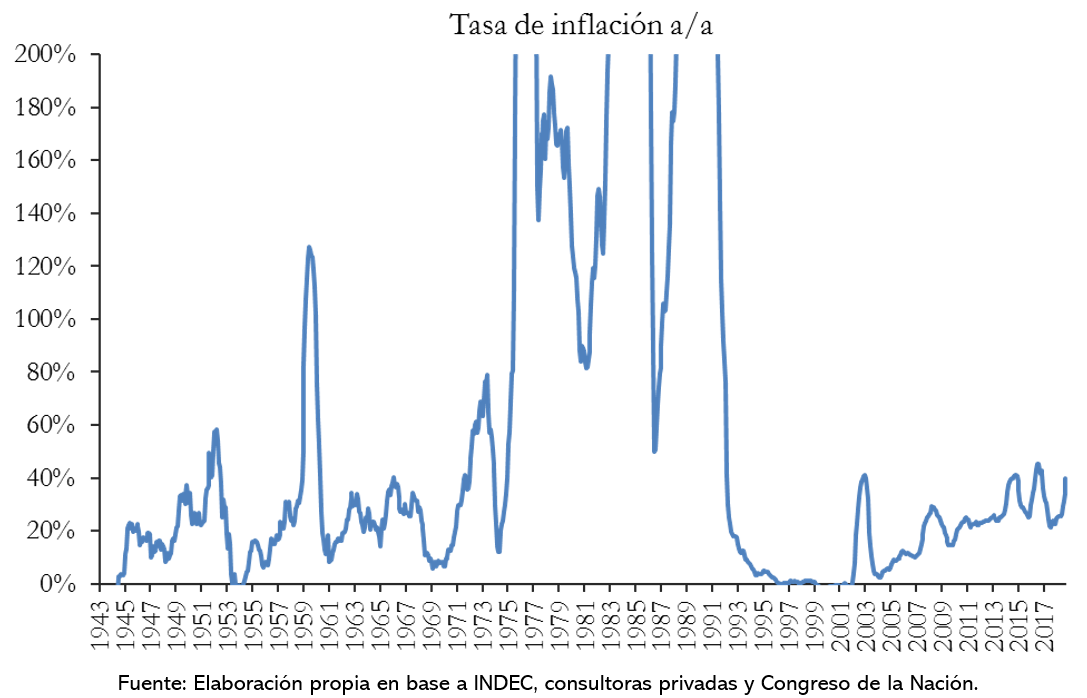
\includegraphics[width=10cm]{Slides Principios de Economia/Figures/P59.png}\
\end{frame}

\begin{frame}{Argentina: crecimiento de M }

\end{frame}

\begin{frame}{Inflación y distribución del ingreso}
    \begin{figure} [H]   
\centering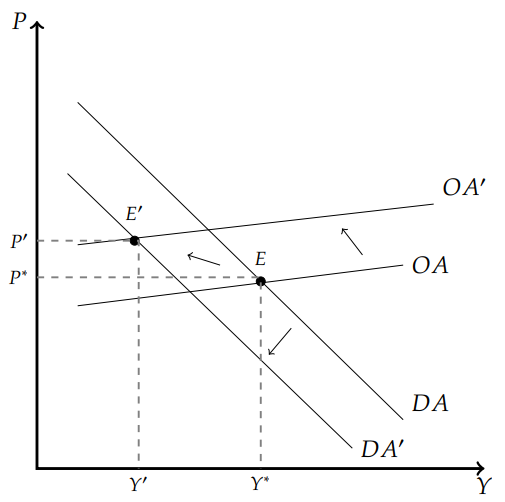
\includegraphics[width=0.9\textwidth]{Slides Principios de Economia/Figures/C33.10.png}\
\caption{\textbf{Efectos redistributivos}}
\end{figure}
\end{frame}


\begin{frame}{}
\centering\huge\textbf{Mercado de dinero} 
\vspace{2mm}
\hrule
\end{frame}

\begin{frame}{Mercado de dinero}
\begin{center}
\begin{figure}[H]
\renewcommand{\figurename}{Figure}
\begin{center}
\begin{tikzpicture}[scale=0.6]
\draw[very thick,<->] (0,11) node[left]{$i$}--(0,0)--(11,0) node[below]{$M$};
\draw[thin] (1,9).. controls (2,3) and (4, 2.5) .. (9, 1.5) node [right]{\footnotesize $M^{d} (P_0,Y_0)$};
\draw[thick](4, 0)--(4, 9) node [above]{\footnotesize $M^{o}$};
\draw[thick,gray, dashed](0,3)--(4,3);
\node[left] at (0,3) {\footnotesize $i_0$};
\node[below] at (4,0) {\footnotesize $M_0$};
\draw[fill](4,3) circle [radius =0.1];
\end{tikzpicture}
\end{center}
\end{figure}
\end{center} 
\end{frame}

\begin{frame}{Movimientos de la demanda de dinero}
\begin{center}
\begin{figure}[H]
\renewcommand{\figurename}{Figure}
\begin{center}
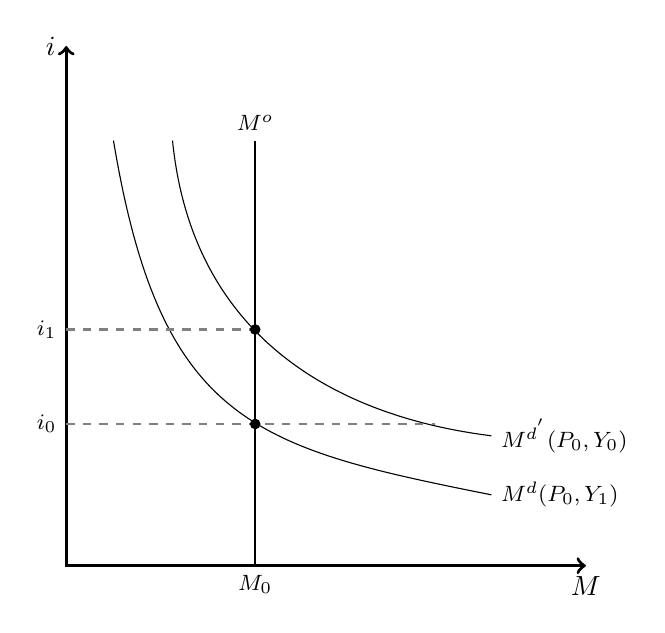
\begin{tikzpicture}[scale=0.6]
\draw[very thick,<->] (0,11) node[left]{$i$}--(0,0)--(11,0) node[below]{$M$};
\draw[thin] (1,9).. controls (2,3) and (4, 2.5) .. (9, 1.5) node [right]{\footnotesize $M^{d} (P_0, Y_1)$};
\draw[thin] (2.25,9).. controls (2.75,4) and (7, 3) .. (9, 2.75) node [right]{\footnotesize $M^{d^{'}} (P_0, Y_0)$};
\draw[thick](4, 0)--(4, 9) node [above]{\footnotesize $M^{o}$};
\draw[thick,gray, dashed](0,3)--(7.8,3);
\node[left] at (0,3) {\footnotesize $i_0$};
\draw[thick,gray, dashed](0,5)--(4,5);
\node[left] at (0,5) {\footnotesize $i_1$};
\node[below] at (4,0) {\footnotesize $M_0$};
\draw[fill](4,3) circle [radius =0.1];
\draw[fill](4,5) circle [radius =0.1];
\end{tikzpicture}
\end{center}
\end{figure}
\end{center} 
\end{frame}


\begin{frame}{Movimientos de la oferta de dinero}
\begin{center}
\begin{figure}[h!]
\renewcommand{\figurename}{Figure}
\begin{center}
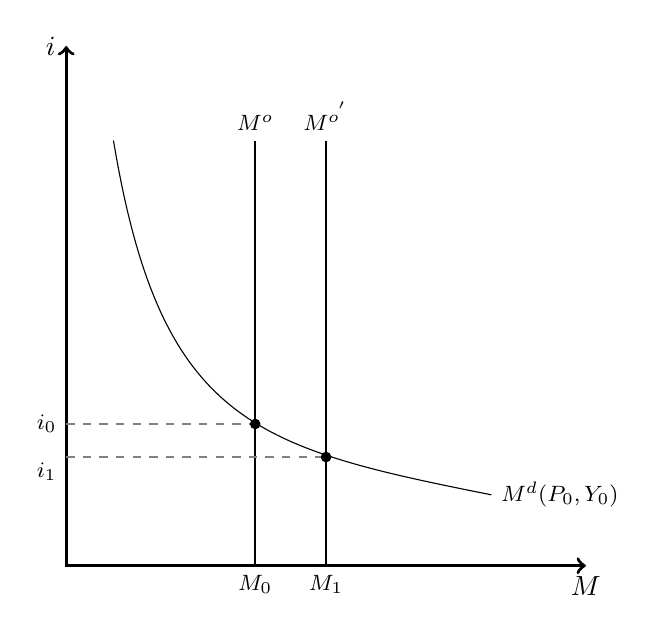
\begin{tikzpicture}[scale=0.6]
\draw[very thick,<->] (0,11) node[left]{$i$}--(0,0)--(11,0) node[below]{$M$};
\draw[thin] (1,9).. controls (2,3) and (4, 2.5) .. (9, 1.5) node [right]{\footnotesize $M^{d} (P_0, Y_0)$};
\draw[thick](4, 0)--(4, 9) node [above]{\footnotesize $M^{o}$};
\draw[thick](5.5, 0)--(5.5, 9) node [above]{\footnotesize $M^{o^{'}}$};
\draw[thick,gray, dashed](0,3)--(4,3);
\node[left] at (0,3) {\footnotesize $i_0$};
\draw[thick,gray, dashed](0,2.3)--(5.5,2.3);
\node[left] at (0,2) {\footnotesize $i_1$};
\node[below] at (4,0) {\footnotesize $M_0$};
\node[below] at (5.5,0) {\footnotesize $M_1$};
\draw[fill](4,3) circle [radius =0.1];
\draw[fill](5.5,2.3) circle [radius =0.1];
\end{tikzpicture}
\end{center}
\end{figure}
\end{center} 
\end{frame}

\begin{frame}{Funcionamiento del mercado monetario}
    \begin{itemize}
    \item La mayoría de los bancos centrales fijan la tasa, pero es lo mismo:
    \end{itemize}
    \vspace{0.4cm}
\begin{center}
\begin{figure}[H]
\renewcommand{\figurename}{Figure}
\begin{center}
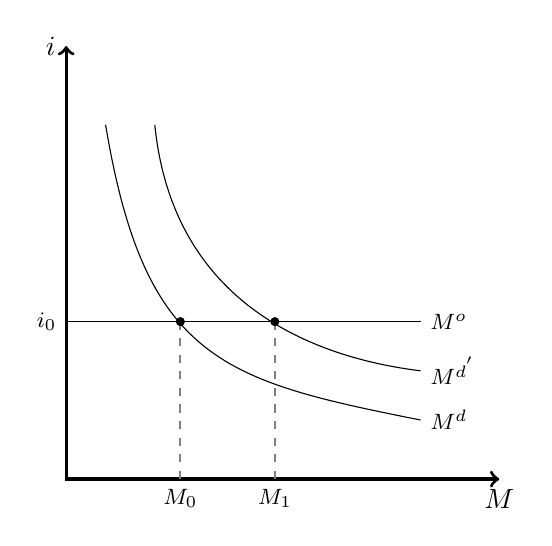
\begin{tikzpicture}[scale=0.5]
\draw[very thick,<->] (0,11) node[left]{$i$}--(0,0)--(11,0) node[below]{$M$};
\draw[thin] (0,4)--(9,4) node[right] {\footnotesize $M^{o}$};
\draw[thin] (1,9).. controls (2,3) and (4, 2.5) .. (9, 1.5) node [right]{\footnotesize $M^{d}$};
\draw[thin] (2.25,9).. controls (2.75,4) and (7, 3) .. (9, 2.75) node [right]{\footnotesize $M^{d^{'}}$};
\node[left] at (0,4) {\footnotesize $i_0$};
\draw[thick,gray, dashed](2.9,0)--(2.9,4);
\draw[thick,gray, dashed](5.3,0)--(5.3,4);
\node[below] at (2.9,0) {\footnotesize $M_0$};
\node[below] at (5.3,0) {\footnotesize $M_1$};
\draw[fill](2.9,4) circle [radius =0.1];
\draw[fill](5.3,4) circle [radius =0.1];
\end{tikzpicture}
\end{center}
\end{figure}
\end{center} 
\end{frame}

\begin{frame}
\frametitle{Tasas de interés}
\begin{itemize}
    \item Tasa de interés nominal $i_t$
    \begin{itemize}
        \item ¿Cómo cambia, en términos de una moneda en particular, el valor de lo que presto o pido prestado? \\
        - Un préstamo de \$V este año genera unos rendimientos de \\ \$(1 + $i_t$)V el próximo año
    \end{itemize} \vspace{4mm}
    \item Tasa de interés real $r_t$
    \begin{itemize}
        \item ¿Qué pasa si hay inflación?
        \item Tasas de interés expresadas en términos de una canasta de bienes \\
        - Tasa que le importa a las personas sin ilusión monetaria
        \end{itemize}
    \end{itemize}
\end{frame}

\begin{frame}
\frametitle{Pensando en la relación}
\begin{itemize}
    \item Entonces tenemos que:\\
    \vspace{2mm}
    \begin{center}
        $1+r_t=(1+i_t)\frac{P_t}{P_{t+1}^{e}}$
    \end{center}
        \vspace{2mm}
    \item Recordemos \\      
    \begin{center}
        $\pi_t=\frac{P_t - P_{t-1}}{P_{t-1}}=\frac{P_t}{P_{t+1}} - 1 $ \\
    \vspace{2mm}
            $\frac{P_t}{P_{t-1}}= \pi_t + 1 $
    \end{center}
\begin{itemize}
    \item Si $\frac{P_t}{P_{t-1}}$ es igual a $(\pi_t + 1)$, podemos establecer:
    \vspace{2mm}
        \begin{center}
            $\frac{P_{t+1}^e}{P_{t}}= \pi_{t+1}^e + 1 $
    \end{center}
\end{itemize} 
\end{itemize}
\end{frame}

\begin{frame}
\frametitle{Intereses e inflación}
\begin{itemize}
    \item Podemos simplificar la relación entre las tasas de interés y la inflación esperada:
    \vspace{2mm}
    \begin{center}
        $1+r_t=\frac{(1+i_t)}{(1+\pi_{t+1}^e)}$
    \end{center}
        \vspace{2mm}
    \item Suponiendo que el valor de las variables no es demasiado grande... $\frac{(1+x)}{(1+y)} \approx 1 + x - y $\\
    - Sabemos que si x, y son pequeñas:     
    \item ... obtenemos la ecuación de Fisher: 
    \vspace{2mm}
        \begin{center}
        $r_t \approx i_t - \pi_{t+1}^e$
    \end{center}
\end{itemize}
\end{frame}


\begin{frame}
\frametitle{Maxi y Gaby}
\begin{itemize}
    \item Maxi le pidió a Gaby \$100 prometiendo pagar \$110, entonces la tasa nominal de interés es:
    \vspace{2mm}
    \begin{center}
        $i_{HOY}=\frac{\$110 - \$100}{\$100} * 100 = 10\%$
    \end{center}
        \vspace{2mm}
    \item Si la tasa de inflación esperada para mañana es 5\%, entonces la tasa de interés real es: \\
    \begin{center}
        $r_{HOY} = i_{HOY}-\pi_{MAÑANA}^e$ \\
        \vspace{2mm}
        $r_{HOY} = 10\%-5\% $ \\
        \vspace{2mm}
        $r_{HOY} = 5\%$
    \end{center}
\end{itemize}
\end{frame}

\begin{frame}{Equilibrio: Mercado monetario y de crédito}
\begin{center}
\begin{figure}[H]
\renewcommand{\figurename}{Figure}
\begin{center}
    \begin{minipage}[b]{0.45\textwidth}
        \begin{center}
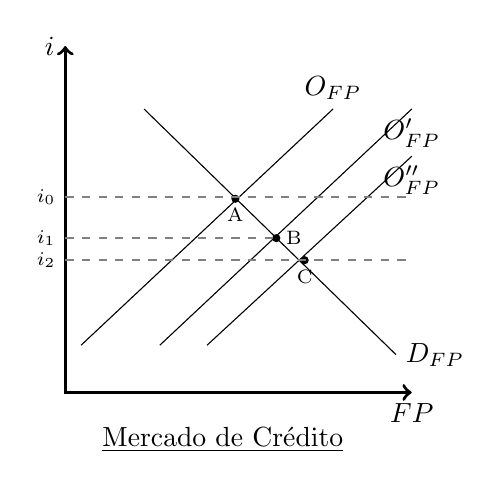
\begin{tikzpicture}[scale=0.4]
\draw[very thick,<->] (0,11) node[left]{$i$}--(0,0)--(11,0) node[below]{$FP$};
\node[] at(5,-1.5) {\underline{Mercado de Crédito}};
\node[left] at(0,6.2) {\scriptsize $i_0$};
\node[left] at(0,4.9) {\scriptsize $i_1$};
\node[left] at(0,4.2) {\scriptsize $i_2$};
\draw[thin](0.5,1.5)--(8.5,9) node [above] {$O_{FP}$};
\draw[thin](3,1.5)--(11,9) node [below] {$O_{FP}'$};
\draw[thin](4.5,1.5)--(11,7.5) node [below] {$O_{FP}''$};
%\draw[thin](2,9)--(10,1.2) node [right] {$D_{FP}$};
\draw[thin](2.5,9)--(10.5,1.2) node [right] {$D_{FP}$};
\draw[fill] (5.4,6.15) circle [radius =0.11] node [below] {\scriptsize A};
\draw[fill] (6.7,4.9) circle [radius =0.11] node [right] {\scriptsize B};
\draw[fill] (7.6,4.2) circle [radius =0.11] node [below] {\scriptsize C};
\draw[thick,dashed,gray] (0,4.9)--(6.7,4.9);
\draw[thick,dashed,gray] (0,4.2)--(11,4.2);
\draw[thick,dashed,gray] (0,6.2)--(11,6.2);
\end{tikzpicture}
\end{center}
     \end{minipage}
  %  \hfill
    \begin{minipage}[b]{0.45\textwidth}
    \begin{center}
\begin{tikzpicture}[scale=0.4]
\draw[very thick,<-] (0,11) node[left]{$i$}--(0,0);
\draw[very thick,->] (0,0)--(11,0) node[below]{$M$};
\node[] at(6,-1.5) {\underline{Mercado de Dinero}};
\draw[thin] (2.75, 9).. controls (3, 7) and (4,2.75) .. (9,2.25) node [right]{\footnotesize $M^{d} (P_0, Y_0)$};
\draw[thin] (3.25, 9).. controls (4, 7) and (5,3) .. (9,3) node [right]{\footnotesize $M^{d^{'}} (P_0, Y_1)$};
\draw[thin] (3.75, 9).. controls (4,7.75) and (5,4) .. (9,3.5);
\node [right] at (9,3.65) {\footnotesize $M^{d^{''}} (P_0, Y_2)$};
\draw[thin](3.5,0)--(3.5,9) node [above]{\footnotesize $M^{o}$};
\draw[thin](7,0)--(7,9) node [above]{\footnotesize $M^{o}'$};
\draw[fill] (3.5,6.25) circle [radius =0.11] node [below left] {\scriptsize A};
\draw[fill] (7,3.45) circle [radius =0.11] node[left] {\scriptsize B};
\draw[fill] (6.9,4.2) circle [radius =0.11] node[above right] {\scriptsize C};
\draw[thick,dashed,gray] (0,4.2)--(11,4.2);
\draw[thick,dashed,gray] (0,6.2)--(11,6.2);
\node[below] at (3.5,0) {\footnotesize $M_0$};
\node[below] at (7,0) {\footnotesize $M_1$};
\draw [thin,gray,decorate,decoration={brace,amplitude=3pt},xshift=0pt,yshift=5pt](3.6,6.3) -- (7,6.3); 
\node[above] at(5.3,6.45) {\scriptsize Gap};
\end{tikzpicture}
\end{center}
    \end{minipage}
\end{center}
\end{figure}
\end{center} 
\end{frame}


\begin{frame}{Equilibrio: Mercado monetario y de crédito}
\begin{center}
\begin{figure}[H]
\renewcommand{\figurename}{Figure}
\begin{center}
    \begin{minipage}[b]{0.45\textwidth}
        \begin{center}
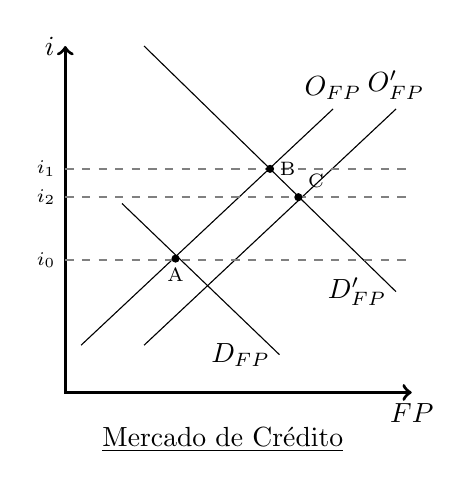
\begin{tikzpicture}[scale=0.4]
\draw[very thick,<->] (0,11) node[left]{$i$}--(0,0)--(11,0) node[below]{$FP$};
\node[] at(5,-1.5) {\underline{Mercado de Crédito}};
\node[left] at(0,4.2) {\scriptsize $i_0$};
\node[left] at(0,7.1) {\scriptsize $i_1$};
\node[left] at(0,6.2) {\scriptsize $i_2$};
\draw[thin](0.5,1.5)--(8.5,9) node [above] {$O_{FP}$};
\draw[thin](2.5,1.5)--(10.5,9) node [above] {$O_{FP}'$};
%\draw[thin](3,1.5)--(11,9) node [below] {$O_{FP}'$};
%\draw[thin](4.5,1.5)--(11,7.5) node [below] {$O_{FP}''$};
\draw[thin](1.8,6)--(6.8,1.2) node [left] {$D_{FP}$};
%\draw[thin](1.5,8)--(8.5,1.2) node [above] {$D_{FP}''$};
\draw[thin](2.5,11)--(10.5,3.2) node [left] {$D_{FP}'$};

\draw[thick,dashed,gray] (0,4.2)--(11,4.2);
\draw[thick,dashed,gray] (0,6.2)--(11,6.2);
\draw[thick,dashed,gray] (0,7.1)--(11,7.1);


\draw[fill] (6.5,7.1) circle [radius =0.11] node [right] {\scriptsize B};
\draw[fill] (7.4,6.2) circle [radius =0.11] node [above right] {\scriptsize C};
\draw[fill] (3.5,4.25) circle [radius =0.11] node [below] {\scriptsize A};
\end{tikzpicture}
\end{center}
     \end{minipage}
  %  \hfill
    \begin{minipage}[b]{0.45\textwidth}
    \begin{center}
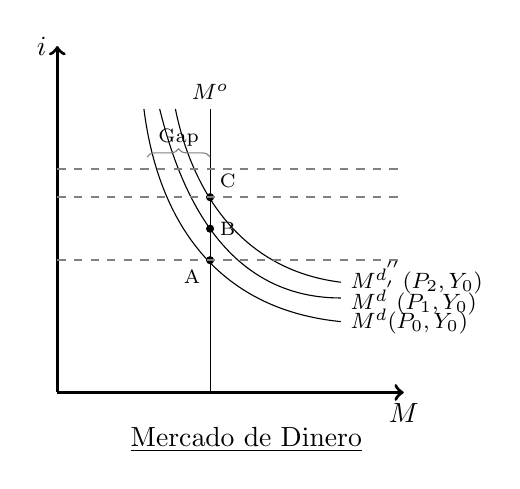
\begin{tikzpicture}[scale=0.4]
\draw[very thick,<-] (0,11) node[left]{$i$}--(0,0);
\draw[very thick,->] (0,0)--(11,0) node[below]{$M$};
\node[] at(6,-1.5) {\underline{Mercado de Dinero}};
\draw[thin] (2.75, 9).. controls (3, 7) and (4,2.75) .. (9,2.25) node [right]{\footnotesize $M^{d}  (P_0, Y_0)$};
\draw[thin] (3.25, 9).. controls (3.75, 7) and (5,3) .. (9,3) node [right]{\footnotesize $M^{d^{'}}  (P_1, Y_0)$};
\draw[thin] (3.75, 9).. controls (4,7.75) and (5,4) .. (9,3.5);
\node [right] at (9,3.65) {\footnotesize $M^{d^{''}}  (P_2, Y_0)$};
\draw[thin](4.85,0)--(4.85,9) node [above]{\footnotesize $M^{o}$};
\draw[fill] (4.85,5.2) circle [radius =0.11] node [right] {\scriptsize B};
\draw[fill] (4.85,4.2) circle [radius =0.11] node[below left] {\scriptsize A};
\draw[fill] (4.85,6.2) circle [radius =0.11] node[above right] {\scriptsize C};
\draw[thick,dashed,gray] (0,4.2)--(11,4.2);
\draw[thick,dashed,gray] (0,6.2)--(11,6.2);
\draw[thick,dashed,gray] (0,7.1)--(11,7.1);

\draw [thin,gray,decorate,decoration={brace,amplitude=3pt},xshift=0pt,yshift=5pt](2.85,7.3) -- (4.85,7.3); 
\node[above] at(3.85,7.5) {\scriptsize Gap};


\end{tikzpicture}
\end{center}
    \end{minipage}
\end{center}
\end{figure}
\end{center} 

\end{frame}

\end{document}



